\chapter{Teorema de Hahn-Banach}

\begin{definicion}
    Sea $X$ un espacio vectorial real, $p: X \to \mathbb{R}$ se dice \textbf{sub-lineal} (o sub-aditiva) si se cumple:
    \begin{itemize}
        \item[i)] $p(x+y) \leq p(x) + p(y) \quad \forall x, y \in X$
        \item[ii)] $p(\alpha x) = \alpha p(x) \quad \forall \alpha \in \mathbb{R}^+, \forall x \in X$
    \end{itemize}
\end{definicion}

\begin{ejemplo}
    Las normas son sub-lineales. \\
\end{ejemplo}

\begin{definicion}
    Un conjunto $X$ está \tbf{totalmente ordenado} si existe una relación binaria $\leq$ que cumple tres propiedades para todos los elementos $a, b, c \in X$:
    \begin{itemize}
        \item[i)] \textbf{Reflexiva:} $a \leq a$
        \item[ii)] \textbf{Antisimétrica:} Si $a \leq b$ y $b \leq a$, entonces $a = b$
        \item[iii)] \textbf{Transitiva:} Si $a \leq b$ y $b \leq c$, entonces $a \leq c$
    \end{itemize}
    Se le dice \tbf{parcialmente ordenado} si la relación $\leq$ no compara todos los elementos de $X$, es decir, pueden existir elementos $x, y \in X$ tales que ni $x \leq y$ ni $y \leq x$.
\end{definicion}

\begin{definicion}
    Sea $(X, \leq)$ un conjunto parcialmente ordenado. Un subconjunto $Y \subseteq X$ se dice \textbf{inductivo} si cada uno de sus subconjuntos totalmente ordenados admite una cota superior, es decir
    \begin{equation*}
        \text{si } Z \subseteq Y \text{ es totalmente ordenado} \implies \exists \alpha \in Y : z \leq \alpha \quad \forall z \in Z
    \end{equation*}
\end{definicion}

\begin{definicion}
    Sea $(X, \leq)$ parcialmente ordenado. Un elemento $m \in X$ se dice \textbf{maximal} si 
    \begin{equation*}
        \forall x \in X \text{ tal que } m \leq x, \text{ entonces } m = x
    \end{equation*}
    es decir, no existe ningún elemento en $X$ que sea mayor que $m$.
\end{definicion}

\begin{ejemplo}
    El conjunto $X = \{ [a, b] \subseteq (0, 1) \subseteq \mathbb{R} \mid a < b \}$ está parcialmente ordenado por la relación de inclusión, veámoslo:
    \begin{itemize}
        \item[i)] \textbf{Reflexiva:} Para todo $[a, b] \in X$, se cumple que $[a, b] \subseteq [a, b]$, por lo tanto $[a, b] \leq [a, b]$.
        \item[ii)] \textbf{Antisimétrica:} Si $[a, b] \leq [c, d]$ y $[c, d] \leq [a, b]$, entonces $[a, b] \subseteq [c, d]$ y $[c, d] \subseteq [a, b]$, lo que implica que $[a, b] = [c, d]$.
        \item[iii)] \textbf{Transitiva:} Si $[a, b] \leq [c, d]$ y $[c, d] \leq [e, f]$, entonces $[a, b] \subseteq [c, d]$ y $[c, d] \subseteq [e, f]$, lo que implica que $[a, b] \subseteq [e, f]$, es decir, $[a, b] \leq [e, f]$.
    \end{itemize}
    En cambio, no es inductivo, ya que el subconjunto $\{ [\frac{1}{n}, 1 - \frac{1}{n} ] \mid n \in \N, n\geq 2 \} \subseteq X$ está ordenado pero no tiene cota superior.
\end{ejemplo}

\begin{lema}(de Zorn)
    Todo conjunto no vacío parcialmente ordenado e inductivo admite un elemento maximal.
\end{lema}


\noindent Los teoremas de Hahn-Banach se ocupan de estudiar las extensiones de aplicaciones lineales definidas en un subespacio $Y$ de un espacio $X$.

\begin{teo}(de Hahn-Banach)
    Sea $X$ un espacio vectorial real y sea $p: X \to \mathbb{R}$ sub-lineal. Sea $Y$ un subespacio vectorial de $X$ y consideramos $f: Y \to \mathbb{R}$ lineal tal que $f(y) \leq p(y)$ para todo $y \in Y$. Entonces: existe $F: X \to \mathbb{R}$ lineal tal que:

    \begin{itemize}
        \item[i)] $F(y) = f(y) \quad \forall y \in Y$
        \item[ii)] $F(x) \leq p(x) \quad \forall x \in X$
    \end{itemize}
\begin{proof}
    La demostración se basa en el Lema de Zorn, veámosla. Sea $\mathcal{F}$ el conjunto de pares $(Y_\alpha, f_\alpha)$ donde:
    \begin{itemize}
        \item[i)] $Y_\alpha \subseteq X$ y $Y \subseteq Y_\alpha$ es un subespacio de $Y_\alpha$.
        \item[ii)] $f_\alpha: Y_\alpha \to \mathbb{R}$ es una extensión lineal de $f$ en $Y_\alpha$.
        \item[iii)] $f_\alpha \leq p$ sobre $Y_\alpha$.
    \end{itemize}
    Sabemos que $\mathcal{F} \neq \emptyset$, de hecho $(Y, f) \in \mathcal{F}$. Definimos una relación de orden en $\mathcal{F}$:
    \begin{equation*}
        (Y_\alpha, f_\alpha) \leq (Y_\beta, f_\beta) \iff Y_\alpha \subseteq Y_\beta, \text{ y } f_\beta \text{ es extensión lineal de } f_\alpha
    \end{equation*}
    $(\mathcal{F}, \leq)$ es un conjunto parcialmente ordenado. Demostremos que $(\mathcal{F}, \leq)$ es inductivo, veámoslo. \\ \\
    \noindent
    Sea $\mathcal{G} \subseteq \mathcal{F}$ una familia totalmente ordenada, veamos que admite una cota superior. Definimos 
    $$M = \bigcup_{Y_\alpha \in \mathcal{G}} Y_\alpha, \quad \tilde{f}(y) := f_\alpha(y) \quad \forall \ Y_\alpha \in \mathcal{G}$$
    entonces, vamos a demostrar que efectivamente $(M, \tilde{f})$ es una cota superior de $\mathcal{G}$, veámoslo:
    \begin{itemize}
        \item[i)] $Y_\alpha \subseteq M \quad \forall \ Y_\alpha \in \mathcal{G}$
        \item[ii)] $\tilde{f}$ está bien definida porque si $y \in Y_\alpha \cap Y_\beta$, entonces uno está contenido en el otro y, por lo tanto, uno es extensión del otro.
        \item[iii)] $\tilde{f}$ es lineal: $\tilde{f}(y_1 + y_2) = f_\alpha(y_1 + y_2) = f_\alpha(y_1) + f_\alpha(y_2) = \tilde{f}(y_1) + \tilde{f}(y_2)$
        \item[iv)] $\tilde{f}(y) = f_\alpha(y) \leq p(y) \quad \forall y \in Y$
    \end{itemize}
    Se sigue que $(M, \tilde{f})$ es una cota superior $\implies \mathcal{F}$ es inductivo. Por el lema de Zorn existe $(Z, F) \in \mathcal{F}$ elemento maximal, por lo tanto $F$ es extensión lineal de $f$ con $F \leq p$ en $Z$. Si verificamos que $Z = X$, hemos terminado. \\ \\
    \noindent
    Supongamos por reducción al absurdo, que $Z \subsetneq X$, entonces existe $x_0 \in X \setminus Z$, y consideramos el subespacio
    \begin{equation*}
        W = \{ z + t x_0 \mid z \in Z, t \in \mathbb{R} \}=Z+\R x_0
    \end{equation*}
    y definimos
    \begin{equation*}
        \phi:W \to \R, \quad \phi(z+tx_0) = F(z) + t c, \quad \forall z \in Z, t \in \R
    \end{equation*}
    donde $c\in \R$ es una constante por determinar. Tenemos que $\phi$ es una extensión lineal de $F$ a $W$, es decir, $\phi|_Z = F$. Para que $\phi$ sea una extensión de $F$ tal que $\phi \leq p$ en $W$, es necesario y suficiente que se cumpla
    \begin{equation} \label{eq:demo-banach}
        \phi(z+tx_0) = F(z) + t c \leq p(z + t x_0) \quad \forall z \in Z, t \in \R
    \end{equation}
    Lo que haremos es ver que necesitamos de $c$ para que se cumpla la desigualdad nombrada anteriormente. Primero cogeremos factor comun de $t$ en la desigualdad, y como trabajamos con funciones lineales y sub-lineales aplicando su propiedad para escalares obtenemos lo siguiente
    \begin{equation*}
        t\left[ F\left(\dfrac{z}{t}\right)+c\right] \leq t p\left(\dfrac{z}{t}+ x_0\right) \quad \forall t \in \R
    \end{equation*}
    y tenemos dos casos:
    \begin{itemize}
        \item Si $t > 0 \implies F\left(\dfrac{z}{t}\right)+c \leq p\left(\dfrac{z}{t}+ x_0\right) \ \forall z \in Z$.
        \item Si $t < 0 \implies F\left(-\dfrac{z}{t}\right)-c \geq p\left(-\dfrac{z}{t}- x_0\right) \ \forall z \in Z$
        \item Si $t = 0$ no se podría haber sacado factor común, pero en este caso la desigualdad \ref{eq:demo-banach} se cumple porque $F(z) \leq p(z)$ para todo $z \in Z$.
    \end{itemize}
    Ahora si tomamos $x=\dfrac{z}{t}$ y $y=-\dfrac{z}{t}$, entonces $x,y \in Z$ y tenemos que $c$ debe cumplir
    \begin{equation*}
        F(x)+c \leq p(x+ x_0) \quad \text{y} \quad F(y)-c \leq p(y- x_0) \implies F(y)-p(y- x_0)\leq c \leq p(x+ x_0)-F(x) 
    \end{equation*}
    Por lo tanto, $c$ debe cumplir la siguiente desigualdad
    \begin{equation*}        
        F(y)-p(y- x_0)\leq c \leq p(x+ x_0)-F(x) \quad \forall x,y \in Z
    \end{equation*}
    notar que aqui hemos generalizado la desigualdad para cualesquiera $x,y \in Z$, ya que $x$ e $y$ dependen de $z$ y $t$, y $z$ es un elemento arbitrario de $Z$ y $t$ es un escalar arbitrario. Sabiendo que $F$ esta dominada por $p$ (lo vimos antes), tenemos que
    \begin{align*}
        F(x)+F(y)=F(x+y) &\leq p(x+y) = p(x+x_0+y-x_0) \leq p(x+x_0)+p(y-x_0) \implies \\
        & \implies F(y)-p(y- x_0)\leq p(x+ x_0)-F(x) \quad \forall x,y \in Z
    \end{align*}
    Nuestro objetivo ahora es ver si realmente existe ese $c$, puesto que hemos encontrado las restricciones que debe cumplir, pero no sabemos si puede existir. Para ellos definimos los dos conjuntos siguientes
    \begin{equation*}
        A = \{ F(y)-p(y- x_0) \mid y \in Z \} \quad \text{y} \quad B = \{ p(x+ x_0)-F(x) \mid x \in Z \}
    \end{equation*}
    y hemos visto que $c$ debe cumplir $a \leq c \leq b$ para todo $a \in A$ y $b \in B$. Por lo tanto, si $\sup A \leq \inf B$, entonces existe tal $c$. Veamos que esto es cierto. Para todo $a \in A$ y $b \in B$, existen $x,y \in Z$ tales que $a = F(y)-p(y- x_0)$ y $b = p(x+ x_0)-F(x)$. Entonces, como hemos visto antes, se cumple que $a \leq b$. Por lo tanto, $\sup A \leq \inf B$, lo que implica que existe tal $c$. Esto demuestra que $\phi$ es una extensión de $F$ a $W$ tal que $\phi \leq p$ en $W$. Por lo tanto
    \begin{equation*}
        (W, \phi) \in \mathcal{F} \quad \text{y} \quad (Z, F) \leq (W, \phi)
    \end{equation*}
    pero como $(Z, F)$ es maximal, entonces $(Z, F) = (W, \phi)$, entonces
    \begin{equation*}
        Z = W = Z + tx_0 \iff x_0 \in Z
    \end{equation*}
    lo que es una contradicción, ya que $x_0 \in X \setminus Z$. Por lo tanto, $Z = X$, lo que implica que $F$ es una extensión lineal de $f$ a $X$ tal que $F \leq p$ en $X$, como se pedía.  \\
\end{proof}
\end{teo}
\noindent
Aplicando esto a los espacios normados, obtenemos el siguiente resultado.

\section{Formulación analítica del teorema de Hahn-Banach}

\begin{teo}(Hahn-Banach analítico)
    Sea $X$ un espacio normado, $Y$ un subespacio de $X$ y sea $f\in Y^*$, entonces existe $F \in X^*$ tal que \begin{itemize}
        \item [i)] $F(y) = f(y) \quad \forall y \in Y$
        \item [ii)] $\|F\| = \|f\|$
    \end{itemize}
\begin{proof}
    Sea $p(x) = \|f\| \cdot \|x\|$, entonces $p$ es sub-lineal por ser multiplicación de normas (la aplicación sub-lineal por excelencia) y domina a $f$, como se ve a continuación
    \begin{equation*}
        f(y) \leq |f(y)| \leq \|f\| \cdot \|y\| = p(y) \quad \forall y \in Y
    \end{equation*}
    Entonces, por el teorema de Hahn-Banach, existe $F: X \to \mathbb{R}$ tal que $F|_Y = f$ y $F(x) \leq p(x)$ para todo $x \in X$. Entonces 
    $$\|F\| = \sup_{\|x\|=1} |F(x)| \leq \sup_{\|x\|=1} p(x) = \sup_{\|x\|=1} \|f\|\cdot\|x\| = \|f\|$$
    Por otro lado
    $$\|F\| = \sup_{\|x\|=1} |F(x)| \geq \sup_{\substack{\|y\|=1 \\ y \in Y}} |F(y)| = \sup_{\substack{\|y\|=1 \\ y \in Y}} |f(y)| = \|f\|$$
    Por lo tanto, $\|F\| = \|f\|$. \\
\end{proof}
\end{teo}

\noindent 
Veamos algunas aplicaciones. \\

\begin{coro}\label{coro:hahn-banach-analitico}
    Sea $X$ un espacio normado y sea $x_0 \in X$, entonces
    \begin{equation*}
        \exists F \in X^* \text{ tal que } F(x_0) = \|x_0\| \text{ y } \|F\| = 1
    \end{equation*}

\begin{proof}
    Sea $Y = \langle x_0 \rangle$ el subespacio generado por $x_0$, y definamos $f: Y \to \mathbb{R}$ por $f(k x_0) = |k| \cdot \|x_0\|$. Entonces, $f$ es lineal y $\|f\| = 1$. Por el teorema de Hahn-Banach, existe $F: X \to \mathbb{R}$ tal que $F|_Y = f$ y $\|F\| = 1$. En particular, $F(x_0) = f(x_0) = \|x_0\|$. \\
\end{proof}
\end{coro}

\begin{coro}
    Sea $(X, \|\cdot\|)$ un espacio normado y sean $x_1, x_2 \in X$ con $x_1 \neq x_2$, entonces
    \begin{equation*}
        \exists F \in X^* \text{ tal que } F(x_1) \neq F(x_2)
    \end{equation*}

\begin{proof}
    Sea $F\in X^*$ tal que $F(x_1 - x_2) = \|x_1 - x_2\|$, podemos encontrar dicha función por el Corolario \ref{coro:hahn-banach-analitico}, entonces como $F$ es lineal, $F(x_1 - x_2) = F(x_1) - F(x_2)$, de lo cual se sigue que
    \begin{equation*}        
        F(x_1) = F(x_2) + \|x_1 - x_2\| \neq F(x_2)
    \end{equation*}
\end{proof}
\end{coro}

\begin{coro}\label{coro:hahn-banach-analitico-norma}
    Sea $(X, \|\cdot\|)$ un espacio normado, entonces para todo $x \in X$ se cumple
    \begin{equation*}
        \|x\| = \sup_{\substack{\|f\|=1 \\ f \in X^*}} |f(x)| \quad \left( = \max_{\substack{\|f\|=1 \\ f \in X^*}} |f(x)| \right)
    \end{equation*}

\begin{proof}
    Sea $f \in X^*$ con $\|f\| = 1$, entonces $|f(x)| \leq \|f\| \cdot \|x\| = \|x\| \implies |f(x)| \leq \|x\|$.
    Por lo tanto:
    \begin{equation*}
        \sup_{\|f\|=1} |f(x)| \leq \|x\|
    \end{equation*}
    Viceversa, por Hahn-Banach existe $F \in X^*$ tal que $F(x) = \|x\|$ y $\|F\| = 1$. Entonces:
    \begin{equation*}        
        |F(x)| = \|x\| \implies \sup_{\|f\|=1} |f(x)| \geq \|x\|
    \end{equation*}
    Se sigue que:
    \begin{equation*}        
        \sup_{\|f\|=1} |f(x)| = \|x\|
    \end{equation*}
\end{proof}
\end{coro}

\begin{coro}\label{coro:hahn-banach-analitico-no-denso}
    Sea $(X, \|\cdot\|)$ un espacio normado y sea $Y \subseteq X$ un subespacio no denso en $X$. Entonces existe $F \in X^*$ tal que:
    \begin{equation*}
        \|F\| = 1 \quad \text{y} \quad F = 0 \text{ en } Y
    \end{equation*}

\begin{proof}
    Sea $Y \subsetneq X$ no denso, entonces $\bar{Y} \subsetneq X$, por lo tanto, existe $x_0 \in X \setminus \bar{Y}$. Sea $Z = \langle x_0, \bar{Y} \rangle$ el subespacio que contiene a $Y$, es decir:
    \begin{equation*}
        Z = \{ k x_0 + y \mid k \in \mathbb{R}, y \in Y \}
    \end{equation*}
    Definimos $f(z) = f(t x_0 + y) = t d(x_0, \bar{Y})$, donde $f: Z \to \mathbb{R}$. Veámos que $f$ es lineal
    \begin{equation*}
        f(z_1 + z_2) = f((t_1 + t_2)x_0 + (y_1 + y_2)) = (t_1 + t_2) d(x_0, \bar{Y}) = f(z_1) + f(z_2)
    \end{equation*}
    Tenemos que $f$ cumple que 
    \begin{equation*}
        f(x_0) = d(x_0, \bar{Y}) \quad \text{y} \quad f(y) = 0 \quad \forall y \in \bar{Y}
    \end{equation*}
    Calculemos finalmente la norma de $f$:
    \begin{equation*}
        |f(z)| = |f(k x_0 + y)| = |t| d(x_0, \bar{Y}) \overset{(*)}{\leq} |t| \left\| x_0 + \frac{y}{t} \right\| = \|t x_0 + y\| = \|z\| \implies \|f\| \leq 1
    \end{equation*}
    donde en $(*)$ hemos usado que podemos elegir $y'=-\frac{y}{t} \in Y$ arbitrario, ya que 
    \begin{equation*}
        d(x_0, \bar{Y}) = \inf_{y' \in \bar{Y}} \|x_0 - y'\| \leq \|x_0 - (-\frac{y}{t})\| = \left\| x_0 + \frac{y}{t} \right\|
    \end{equation*}
    Sea $(y_n) \in \bar{Y}$ una sucesión tal que $d(x_0, y_n) \to d(x_0, \bar{Y})$, por lo tanto
    \begin{align*}
        d(x_0, \bar{Y}) &= f(x_0) = f(x_0) - \underbrace{f(y_n)}_{0} = f(x_0 - y_n) \leq \\
        &\leq |f(x_0 - y_n)| \leq \|f\| \cdot \|x_0 - y_n\| = \|f\| \cdot d(x_0, y_n)
    \end{align*}
    y cuando $n \to \infty$, se tiene 
    \begin{equation*}
        d(x_0, \bar{Y}) \leq \|f\| \cdot d(x_0, y_n) \to \|f\| \cdot d(x_0, \bar{Y}) \implies \|f\| \geq 1
    \end{equation*}
    y, por lo tanto, se sigue que $\|f\| = 1$. Por el teorema de Hahn-Banach existe $F: X \to \mathbb{R}$ tal que $\|F\| = \|f\|=1$ y $F|_Z = f$. En particular, $F(y) = f(y) = 0$ para todo $y \in Y$, como se quería demostrar. \\
\end{proof}
\end{coro}

\begin{ejercicio}
    Sea $X$ un espacio normado, entonces para $x\in X$ se cumple 
    \begin{equation*}
        x =  0 \iff f(x) = 0 \quad \forall f \in X^* \\
    \end{equation*}
    \begin{description}
        \item[$\implies)$] Obvio, si $x = 0$, entonces $f(x) = f(0) = 0$ para todo $f \in X^*$, por linealidad de $f$.
        \item[$\impliedby)$] Supongamos que $x \neq  0 $, entonces existe $x_0 \in X$ con $x_0 \neq 0$. Por el Corolario \ref{coro:hahn-banach-analitico}, existe $F \in X^*$ tal que $F(x_0) = \|x_0\| \neq 0$ y $\|F\| = 1$. Por lo tanto, $f(x) \neq 0$ para algún $f \in X^*$, lo que es una contradicción. Por lo tanto, $x = 0$. \\ 
    \end{description}
\end{ejercicio}

\begin{ejercicio}
    Demostrar que si $X^*$ es separable, entonces 
    $$S^* = \{ F \in X^* \mid \|F\| = 1 \} \subseteq X^*$$ 
    es separable. \\

    \noindent
    Antes de comenzar con la demostración, recordemos que un espacio $X$ es separable si tiene un subconjunto denso numerable. Visto de otra manera, existe una sucesión $(x_n) \in X$ tal que $\overline{\{ x_n \}_{n\in \N}} = X$. \\ \\
    \noindent
    Dado que $X^*$ es separable, existe una sucesión (subconjunto numerable) $(f_n) \in X^*$ densa en $X^*$, entonces, el conjunto $\overline{\{f_n\}_{n \in \mathbb{N}} }$ es denso en $X^*$. Por lo tanto, el conjunto 
    \begin{equation*}
        \overline{\left\{\dfrac{f_n}{\|f_n\|}\right\}_{n \in \mathbb{N}}}
    \end{equation*}
    es denso en $S^* = \{ F \in X^* \mid \|F\| = 1 \}$, lo que implica que $S^*$ es separable. \\

    \noindent
    De hecho, podríamos haber tomado el conjunto generado por la sucesión $(f_n) \in X^*$, es decir, el conjunto $[\{f_n\}_{n \in \mathbb{N}}]$ que es el conjunto de todas las combinaciones lineales de los elementos de la sucesión, y luego normalizar cada elemento de ese conjunto, es decir, tomar el conjunto $\left[\left\{ \frac{f_n}{\|f_n\|}_{n \in \mathbb{N}} \right\}\right] $ que claramente es denso. Para ambos conjuntos se es solo numerable si los \tbf{coeficientes son $\Q$}.
\end{ejercicio}

\begin{ejercicio}
    En $l_p$ con $p \in [1, +\infty)$, se puede definir una base de Schauder $e_i = (0, 0, \dots, \underset{i}{1}, 0, \dots, 0)$. \\

    \noindent
    Sea $x \in l_p$, entonces $x$ se puede escribir como $x = \sum\limits_{k=1}^{\infty} x_k e_k$. Sea $x_n = \sum\limits_{k=1}^{n} x_k e_k$, entonces:
    \begin{equation*}
        \|x - x_n\|_p = \left\| \sum_{k=n+1}^{+\infty} x_k e_k \right\|_p \xrightarrow{n \to +\infty} 0. \text{ De lo cual } x_n \to x.
    \end{equation*}
    donde lo que hemos usado es que como $x \in l_p$, entonces $\sum\limits_{k=1}^{\infty} |x_k|^p < +\infty$, lo que implica que $\left(\sum\limits_{k=n+1}^{+\infty} |x_k|^p \right)^\frac{1}{p} \to 0$ cuando $n \to +\infty$. \\

    \noindent
    Se tiene demostrado que es base de Schauder, puesto que la sucesión de escalares es única, ya que viene dada univocuamente por $x\in l_p$ y hemos demostrado el límite.
\end{ejercicio}

\observacion{
    Sea $F\in l_p^*$ (espacio de funciones lineales de vectores de $l_p$), entonces dado que $\{ e_n \}_{n\in \N}$ es base de Schauder, cada $x = \sum\limits_{k=1}^{\infty} x_k e_k$, de lo cual:
    \begin{equation*}
        F(x) := F\left( \sum_{k=1}^{\infty} x_k e_k \right) = \sum_{k=1}^{\infty} x_k F(e_k)
    \end{equation*}
    entonces dado $a_k := F(e_k)$, vemos que la sucesión $a_F = (a_1, a_2, \dots)$ caracteriza el funcional.
}

\section{Espacio dual y reflexivo}

\begin{teo}\label{teo:separable-dual-separable}
    Sea $(X, \|\cdot\|)$ un espacio normado, entonces tenemos que 
    \begin{equation*}
        X^* \text{ es separable} \implies X \text{ es separable}
    \end{equation*}

\begin{proof}
    Sabemos que $X^*$ es separable, por lo tanto, el conjunto $S^* = \{ F \in X^* \mid \|F\| = 1 \}$ es separable (Ejercicio 2). Entonces, existe una sucesión $(f_n) \in S^*$ densa en $S^*$. Para cada $n$, tenemos que 
    \begin{equation*}
        \|f_n\| = \sup_{\|x_n\|=1} |f_n(x_n)| = 1 \implies \exists x_n : |f_n(x_n)| > 1/2 \text{ y } \|x_n\| = 1
    \end{equation*}
    Sea ahora $Y = [\{x_n\}]$ el subespacio generado por la sucesión $(x_n)$, donde los escalares pertenecen a $\Q$, entonces vamos a demostrar que $\bar{Y} = X$, lo que implica que $X$ es separable. \\ \\
    \noindent
    Supongamos por reducción al absurdo que $\bar{Y} \subsetneq X$, entonces por Hahn-Banach existe $G \in X^*$ tal que $\|G\| = 1$ y $G(y) = 0$ para todo $y \in Y$. Entonces, $G(x_n) = 0$ para todo $n$. De lo cual se sigue que
    \begin{equation*}
        |f_n(x_n) - G(x_n)| = |f_n(x_n)| > 1/2 \implies 1/2 < |f_n(x_n) - G(x_n)| \leq \|f_n - G\| \cdot \|x_n\| = \|f_n - G\|
    \end{equation*}
    lo que es una contradicción, porque $\{f_n\}$ es densa en $S^*$, por lo tanto, debe ``acercarse" a $G$. Por lo tanto, $\bar{Y} = X$, lo que implica que $X$ es separable. \\
\end{proof}
\end{teo}

\begin{coro}
    $l_\infty \subsetneq l_1^*$ (de lo contrario sería separable).
\end{coro}

\begin{definicion}
    Sea $(X, \|\cdot\|)$ un espacio normado, entonces el \tbf{espacio dual} de $X$ es el espacio 
    $$X^{**} := \{ F: X^* \to \mathbb{R} \text{ lineales y continuas} \}$$
    La función 
    \Func{J}{X}{X^{**}}{x}{J_x}
    donde $J_x: X^* \to \mathbb{R}$ con $J_x(f) := f(x)$ se llama \textbf{inyección canónica} (o mapeo canónico).
\end{definicion}

\observacion{
    La inyección canónica $J$ es una \tbf{función linear y continua}, veámoslo. Para $x_1, x_2 \in X$ y $t \in \mathbb{R}$, tenemos que
    \begin{equation*}
        J_{x_1 + t x_2}(f) = f(x_1 + t x_2) = f(x_1) + t f(x_2) = J_{x_1}(f) + t J_{x_2}(f)
    \end{equation*}
    lo que demuestra que $J$ es lineal. Para ver la continuidad de $J$, veamos que $J_x$ es continua para cada $x \in X$. Para ello, veamos que $J_x$ es acotada, lo cual implica que es continua. De hecho, para cada $f \in X^*$ se cumple que
    \begin{equation*}
        |J_x f| = |f(x)| \leq \|f\| \cdot \|x\| \implies \|J_x\| = \sup_{\|f\|=1} |J_x f| \leq \sup_{\|f\|=1} \|f\| \cdot \|x\| = \|x\|
    \end{equation*}
    donde tenemos que al ser un operador acotado $J_x$ es continuo para todo $x \in X$, entonces $J$ es continuo. \\
}

\noindent
Siguiendo con la lógica de la observación vamos a demostrar que $J$ es una isometría, es decir, $\|J_x\| = \|x\|$ para todo $x \in X$. Para ello, veamos que $\|J_x\| \leq \|x\|$ (visto en la observación) y $\|J_x\| \geq \|x\|$, veámoslo. \\
\noindent
Por el corolario de Hahn-Banach para cada $x\in X$, tenemos que $\exists f \in X^*$ tal que $f(x) = \|x\|$ y por lo tanto $\|J_x f\| = |f(x)| = \|x\|$. De lo cual
\begin{equation*}
    \|J_x\| = \|x\| \quad \text{y por lo tanto} \quad \|J\| = 1
\end{equation*}
por lo que tenemos que $J$ es una \tbf{isometría}.  \\ \\
\noindent 
Para demostrar la inyectividad de $J$, tenemos que dados $x_1 \neq x_2$, entonces 
\begin{equation*}
    \exists f \in X^* : f(x_1) \neq f(x_2) \implies J_{x_1}(f) \neq J_{x_2}(f)
\end{equation*}
lo que demuestra la \tbf{inyectividad} de $J$. De hecho, tenemos que $J_x$ es isomorfismo lineal, y por tanto 
\begin{equation*}
    X\simeq J(X) \subseteq X^{**}
\end{equation*}

\begin{definicion}
    Sea $(X, \|\cdot\|)$ un espacio normado, entonces se dice $X$ \tbf{reflexivo} si $J: X \to X^{**}$ es sobreyectiva, y por tanto $J$ es un isomorfismo algebraico y topológico.
\end{definicion}

\observacion{
    En general, podrían existir isomorfismos entre $X$ y $X^{**}$ sin que $J$ lo sea.
}

\observacion{
    Si $X$ es reflexivo, entonces $X$ es completo porque $X^{**}$ es completo y, por lo tanto, también $X$ lo es.
}

\begin{ejemplo}
    $L^p$, con $p\in [1, +\infty)$, es reflexivo.
\end{ejemplo}

\begin{prop}
    Sea $X$ un espacio reflexivo, entonces cada subespacio cerrado es también reflexivo.

\begin{proof}
    Sea $J':Y\to Y^{**}$ con $Y$ cerrado, nuestro objetivo es demostrar que $J'$ es sobreyectiva, es decir, que dado $g \in Y^{**}$, existe $y \in Y$ tal que $J'_y = g$. \\
    
    \noindent
    Sea $g \in Y^{**}$ arbitrario, vamos a definir la siguiente aplicación
    \Func{f_g}{X^*}{\R}{F}{f_g(F) = g(F|_Y)}
    donde $F|_Y$ es la restricción de $F$ a $Y$. Está claro que $f_g$ está bien definida, es lineal y continua, por ser restricción de una función lineal y continua, es decir, pertenece a $X^{**}$.\\ \\
    \noindent
    Puesto que $J$ es sobreyectiva, $\exists x \in X$ tal que $J_x = f_g$. Demostremos que $x \in Y$. Supongamos por reducción al absurdo que $x \notin Y=\bar{Y}$ (la igualdad es por ser $Y$ cerrado), entonces por el corolario de Hahn-Banach \ref{coro:hahn-banach-analitico-no-denso} como $Y$ no es denso en $X$, se cumple que
    \begin{equation*}
        \exists \tilde{F} \in X^* \text{ tal que } \tilde{F}|_Y = 0, \|\tilde{F}\| = 1 \text{ y } \tilde{F}(x) = d(x, Y) > 0
    \end{equation*}
    Entonces, $x \notin Y \implies \tilde{F}(x) \neq 0$, pero por otro lado
    $$0 \neq \tilde{F}(x) = J_x(\tilde{F}) = f_g(\tilde{F}) = g(\tilde{F}|_Y) \overset{(**)}{=}g(0) \overset{(*)}{=} 0$$
    donde en $(*)$ hemos usado que $g$ es lineal, y en $(**)$ que $\tilde{F}|_Y = 0$. Esto es una contradicción. Por lo tanto, $x \in Y$, lo que implica que $J'_x = g$, ya que tenemos que 
    \begin{equation*}\label{eq:prop-cerrado-reflexivo}
        F(x)=J_x(F) = f_g(F) = g(F|_Y) \quad \forall F \in X^* \implies J'_x(F') = g(F'|_Y)=g(F') \quad \forall F' \in Y^*
    \end{equation*}
    como se quería demostrar. \\ \\
    \noindent
    Si la explicación de antes de $J'_x=g$ no nos es clara, podemos demostrarlo más rigurosamente, de la siguiente manera. Tomemos $h\in Y^*$ arbitrario, demostraremos que $J'_x(h)=g(h)$, donde
    \Func{J'_x}{Y^{**}}{\R}{h}{h(x)}
    Por el Teorema de Hahn-Banach, sabemos que todo funcional en un subespacio $Y\subseteq X$ puede extenderse a un funcional $F$ en el espacio total $X$ tal que $F|_Y = h$. Como $F$ es la extensión de $h$ y $x \in Y$, entonces $h(x) = F(x)$. \\
    Usando la igualdad del principio de la ecuación \ref{eq:prop-cerrado-reflexivo}, es decir, $F(x)=J_x(F)$, tenemos que
    $$F(x) = g(F|_Y) = g(h)$$
    y finalmente concluimos que $J'_x(h) = h(x)=F(x)=g(h)$.
\end{proof}
\end{prop}

\begin{prop}
    Dado dos espacios normados $X$ e $Y$, y sea $T: X \to Y$ un operador lineal acotado, entonces $T^*$ también lo es y además $\|T^*\|=\|T\|$.
\end{prop}

\begin{prop}[Regla de la composición de adjuntos]
    En general, si tienes dos operadores lineales acotados $A: X \to Y$ y $B: Y \to Z$, el adjunto de la composición cumple que
    $$(B \circ A)^* = A^* \circ B^*$$
\end{prop}

\begin{ejercicio}
    Si $Y$ y $X$ son isomorfos, entonces 
    \begin{equation*}
        X \text{ reflexivo} \iff Y \text{ reflexivo}
    \end{equation*}
    Supongamos $X$ reflexivo, entonces $J: X \to X^{**}$ es sobreyectiva. Sea $T: X \to Y$ un isomorfismo, entonces dado 
    \Func{T^*}{Y^*}{X^*}{g}{T^*(g) = g \circ T}
    tenemos que es un isomorfismo con inversa $(T^{-1})^*$, ya que
    \begin{itemize}
        \item $(T^*)^{-1}\circ T^*=(T^{-1})^* \circ T^* = (T \circ T^{-1})^* = (Id_Y)^* = Id_{Y^*}$
        \item $T^*\circ (T^*)^{-1} = T^* \circ (T^{-1})^* = (T^{-1} \circ T)^* = (Id_X)^* = Id_{X^*}$
    \end{itemize}
    Veámos el siguiente diagrama conmutativo

    \begin{center}
    \shorthandoff{"}
    \begin{tikzcd}
    X \arrow[r, "T"] \arrow[d, "J"'] & Y \arrow[d, "J'"] \\
    X^{**} \arrow[r, "T^{**}"]       & Y^{**}
    \end{tikzcd}
    \shorthandon{"} 
    \end{center}
    
    de donde se deduce que $T^{**}$ es un isomorfismo (podemos pensarlo igual que hemos hecho con $T^*$). Si demostramos que el diagrama conmutativo es válido, habremos terminado, pues tendríamos que $J'$ es sobreyectiva. \\ \\
    \noindent
    Para ello, necesitamos ver que ambos caminos, superior derecha e inferior izquierda, llevan a la misma función. Teniendo lo siguiente
    \begin{equation*}
        T^{**} \circ J(x) = T^{**}(J_x) = J_x \circ T^* \quad \text{y} \quad J' \circ T(x) = J'(T(x)) = J'_{T(x)}
    \end{equation*}
    el objetivo será demostrar que 
    \begin{equation*}
        J'_{T(x)}(F) = J_x \circ T^*(F) \quad \forall F \in Y^*
    \end{equation*}
    De hecho, $J'_{T(x)}(F) = F(T(x))$ y $J_x(T^* F) = J_x(F \circ T) = F \circ T(x)$, lo que demuestra la validez del diagrama conmutativo. Por lo tanto, $J'$ es sobreyectiva, lo que implica que $Y$ es reflexivo. \\
\end{ejercicio}


\begin{prop}
    La propiedad de ser reflexivo se mantiene por isomorfismos.
\end{prop}

\section{Formulación geométrica del teorema de Hahn-Banach}

\begin{definicion}
    Sea $f: X \to \mathbb{R}$ un funcional, entonces el conjunto 
    \begin{equation*}
        \pi_\alpha = \{ x \in X \mid f(x) = \alpha \}
    \end{equation*}
    se llama \textbf{hiperplano} de $X$.
\end{definicion}

\begin{observacion}
    Decimos que $f$ es un funcional, cuando nos referimos a una función cuyo dominio es un espacio vectorial $X$ y cuyo codominio es el cuerpo de los escalares (que en nuestro curso suele ser $\mathbb{R}$, aunque podría ser $\mathbb{C}$). 
\end{observacion}

\begin{definicion}
    Un conjunto $C$ en un espacio vectorial $X$ se dice \textbf{convexo} si, para cualquier par de puntos $x, y \in C$, el segmento que los une también está contenido íntegramente en $C$.  Matemáticamente, esto se traduce en que se cumple que
    \begin{equation*}
        tx + (1-t)y \in C, \quad \forall x, y \in C, \ \forall t \in [0, 1]
    \end{equation*}
    
\end{definicion}

\begin{definicion}
    Sean $A,B$ subconjuntos convexos de un espacio vectorial, entonces se dice que un hiperplano $\pi_\alpha$ \textbf{separa} $A$ y $B$ si
    \begin{equation*}
        f(a) \leq \alpha \leq f(b) \quad \forall a \in A, b \in B
    \end{equation*}
\end{definicion}

\observacion{
    Si $X$ es normado y $f$ es lineal y continua, entonces $\pi_\alpha = f^{-1}(\alpha)$ es cerrado, ya que es la preimagen de un conjunto cerrado por una función continua. De hecho, $\pi_\alpha$ es un hiperplano cerrado. \\
}

\begin{teo}[Teorema de Hahn-Banach geométrico]\label{teo:hahn-banach-geometrico}
    Sea $X$ un espacio normado y sean $A, B$ convexos disjuntos no vacíos. Si $A$ es abierto, entonces 
    \begin{equation*}
        \exists f \in X^* \text{ y } \alpha \in \mathbb{R} \text{ tales que } \pi_\alpha^f = \{ f = \alpha \} \text{ separa } A \text{ y } B
    \end{equation*}
\end{teo}

\begin{coro}
    Sea $C$ cerrado y convexo con interior no vacío ($C^\circ \neq \emptyset$) de un espacio normado $X$, entonces 
    \begin{equation*}
        \forall b \in \partial C, \ \exists f \in X^* \text{ tal que } f(x) \leq f(b) \quad \forall x \in C
    \end{equation*}

\begin{proof}
    Sea $A = C^\circ\neq \emptyset$, podemos ver fácilmente si es convexo, tomando $x,y\in A$, y sea \mbox{$t\in [0,1]$} arbitrario, tenemos $z=tx+(1-t)y$. Por definición de abierto, tenemos que $\exists r_x, r_y > 0$ tales que $B(x, r_x) \subseteq C$ y $B(y, r_y) \subseteq C$. Entonces, si tomamos $r = \min\{r_x, r_y\}$, entonces $B(x, r) \subseteq C$ y $B(y, r) \subseteq C$. Por lo tanto, 
    \begin{equation}
        B(z,r)=z+B(0,r) = t(x+B(0,r))+(1-t)(y+B(0,r)) \subseteq tC+(1-t)C = C
    \end{equation}
    donde lo que hemos usado es aplicar la propiedad de convexidad de $C$ a los conjuntos $x+B(0,r)$ y $y+B(0,r)$, que son subconjuntos de $C$. \\

    \noindent    
    Por otra parte, tenemos $B = \{b\}$ con $b \in \partial C$, entonces $A \cap B = \emptyset$ son convexos y, por lo tanto, aplicando Teorema \ref{teo:hahn-banach-geometrico} $\exists f \in X^*, \alpha \in \mathbb{R}$ tales que:
    \begin{equation*}
        f(x) \leq \alpha \leq f(b) \quad \forall x \in C^\circ
    \end{equation*}
    Además, para $b\in \partial C$, tenemos $f(b)\leq f(b)$, por lo que dado que $C$ es cerrado, entonces \mbox{$C = C^\circ \cup \partial C$}, y por lo tanto, $f(x) \leq f(b)$ para todo $x\in C$. \\
\end{proof}
\end{coro}

\begin{definicion}
    Sea $A \subseteq X$ un subconjunto de un espacio normado $X$. Se dice que $A$ está \tbf{todo de un lado} respecto a $\pi_\alpha^{(f)}$ si
    \begin{equation*}
        f(x) \leq \alpha \quad \forall x \in A \quad \text{o bien} \quad f(x) \geq \alpha \quad \forall x \in A
    \end{equation*}
    Si existe $b \in A$ tal que $f(b) = \alpha$, entonces $\pi_\alpha$ se llama \textbf{hiperplano de soporte} y $f$ se llama \textbf{función de soporte}. Podemos ver un ejemplo representativo en la Figura \ref{fig:hiperplano-soporte}.
\end{definicion}

\begin{figure}
    \centering
    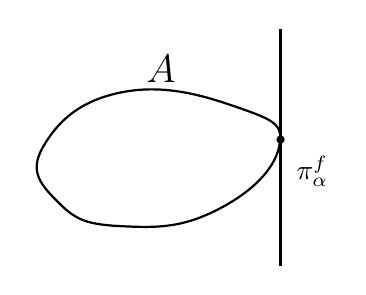
\begin{tikzpicture}
        % Dibujo del conjunto convexo A (forma irregular pero suave)
        \draw[thick] plot [smooth cycle, tension=0.8] coordinates {
            (0,0.5) (1,1.2) (2.5,1) (3,0.5) (2.2,-0.3) (1,-0.5) (0.2,-0.2)
        };
        
        % Etiqueta del conjunto A
        \node at (1.5,1.5) {\Large $A$};
        
        % Dibujo del hiperplano de soporte (línea vertical f = alpha)
        % El punto de contacto está aproximadamente en x = 3
        \draw[very thick] (3.02,-1) -- (3.02,2);
        
        % Etiqueta de la función de soporte f = alpha
        \node[right] at (3.1,0.2) {$\pi_\alpha^f$};
        
        % Punto de tangencia (opcional, para mayor precisión)
        \fill (3.02,0.6) circle (1.5pt);

    \end{tikzpicture}
    \caption{Ejemplo de un conjunto convexo $A$ y un hiperplano de soporte $\pi_\alpha^f$.}
    \label{fig:hiperplano-soporte}
\end{figure}

\begin{teo}[Teorema de Hahn-Banach fuerte]\label{teo:hahn-banach-fuerte}
    Sean $A, B$ conjuntos convexos no vacíos, con $A$ cerrado y $B$ compacto en un espacio normado $X$. Entonces existen $\alpha, \beta$ reales con $\alpha < \beta$ y $f \in X^*$ tales que
    \begin{equation*}
        f(a) \leq \alpha < \beta \leq f(b) \quad \forall a \in A, b \in B
    \end{equation*}
    Por lo tanto, el intervalo $(\alpha, \beta)$ separa los dos conjuntos.
\end{teo}

\section{Integración en espacios de Banach}


\noindent 
Sea $\varphi: [0, 1] \to X$ continua. Queremos definir $\int_{0}^{1} \varphi(t) dt$. \\

\noindent 
Sea $P$ una partición de $[0, 1]$, es decir, $P = \{0 = t_0 < t_1 < \dots < t_n = 1\}$. Definimos las sumas integrales $\sigma_n$ como
\[ \sigma_n := \sum_{i=1}^{n} \varphi(\xi_i)(t_i - t_{i-1}) \quad \text{con } \xi_i \in [t_{i-1}, t_i]. \]

\vspace{0.4cm}

\noindent 
Tiene sentido definir $\varphi$ como integrable si existe $\lim\limits_{n \to +\infty} \sigma_n =: y \in X$. Supongamos que $y$ existe, veamos qué propiedades tiene. \\

\noindent 
Sea $f \in X^*$, entonces 
\begin{equation*}
    f(y)=f\left(\lim_{n\to +\infty}\sigma_n\right) \overset{(*)}{=} \lim_{n\to + \infty} f(\sigma_n) \overset{(**)}{=} \lim_{n \to +\infty} \sum_{i=1}^{n} f(\varphi(\xi_i))(t_i - t_{i-1})
\end{equation*}
donde en $(*)$ hemos usado que $f$ continua y en $(**)$ que es lineal. Además, como
$f \circ \varphi: [0, 1] \to \mathbb{R}$ es continua, si existe $y$, podemos definir 

$$f(y) = \int_{0}^{1} f(\varphi(t)) dt$$
que obviamente está bien definido porque $f \circ \varphi$ es continua por composición de continuas. Por lo tanto
$$f\left( \int_{0}^{1} \varphi(t) dt \right) = \int_{0}^{1} f \circ \varphi(t) dt \quad \forall f \in X^*$$
donde hemos usado la conmutatividad entre el funcional lineal y la integral.

\begin{definicion}
    Sea $\varphi: [0, 1] \to X$ continua. Definimos la integral $\varphi$ en $X$ como el \tbf{único elemento} $y \in X$ tal que 
    $$f(y) = \int_{0}^{1} f \circ \varphi(t) dt \quad \forall f \in X^*$$
    En este caso lo llamamos 
    $$y := \int_{0}^{1} \varphi(t) dt$$
\end{definicion}

\observacion{
    No hemos demostrado la existencia de $y$, pero veámos la unicidad. Sean $y_1, y_2 \in X$ tales que $f(y_1) = f(y_2) \quad \forall f \in X^*$, entonces $f(y_1 - y_2) = 0 \quad \forall f \in X^*$. Aplicando el \mbox{Corolario \ref{coro:hahn-banach-analitico-norma}}, tenemos que 
    \begin{equation*}
        \|y_1 - y_2\| = \sup_{\substack{\|f\|=1 \\ f \in X^*}} |f(y_1 - y_2)| \overset{(*)}{=} 0 \implies y_1 - y_2 = 0 \implies y_1 = y_2\sup_{\|f\|=1 \\ f\in X^*} 
    \end{equation*}
    donde en $(*)$ hemos usado que $f(y_1 - y_2) = 0$ para todo $f \in X^*$. Por lo tanto, la integral de $\varphi$ es única.
}

\begin{prop}
    Si $\varphi: [0, 1] \to X$ es continua, entonces 
    \begin{equation*}
        \left\| \int_{0}^{1} \varphi(t) dt \right\| \leq \int_{0}^{1} \|\varphi(t)\| dt
    \end{equation*}

\begin{proof}
    Sea $y = \int_{0}^{1} \varphi(t) dt$, entonces por Corolario \ref{coro:hahn-banach-analitico} tenemos que
    \begin{equation*}
        \exists f\in X^* \text{ tal que } f(y) = \|y\| \text{ y } \|f\| = 1
    \end{equation*}
    entonces
    \begin{align*}
        |f(y)| = \|y\| &= \left\| \int_{0}^{1} \varphi(t) dt \right\| = \left| f \int_{0}^{1} \varphi(t) dt \right| = \left| \int_{0}^{1} f \circ \varphi(t) dt \right| \leq \int_{0}^{1} |f \circ \varphi| dt = \\
        &= \int_{0}^{1} |f(\varphi(t))| dt \leq \int_{0}^{1} \underbrace{\|f\|}_{1} \cdot \|\varphi(t)\| dt \leq \int_{0}^{1} \|\varphi(t)\| dt \quad \square
    \end{align*}
\end{proof}
\end{prop}



\noindent Si $\varphi: [a, b] \to X$ de forma análoga: $f\left( \int_{a}^{b} \varphi(t) dt \right) = \int_{a}^{b} f \circ \varphi(t) dt \quad \forall f \in X^*$.

\vspace{0.4cm}

\noindent Si $\varphi: [a, +\infty) \to X$, entonces $\int_{a}^{+\infty} \varphi(t) dt := \lim\limits_{b \to +\infty} \int_{a}^{b} \varphi(t) dt$ y
\[ f\left( \int_{a}^{+\infty} \varphi(t) dt \right) = \int_{a}^{+\infty} f \circ \varphi(t) dt \quad \forall f \in X^* \] \\

\noindent
En resumen la integral definida para funciones con valores en un espacio de Banach (a menudo llamada \tbf{integral de Bochner o de Riemann-Banach}) hereda las propiedades fundamentales del cálculo integral clásico de funciones reales, es decir, 

$$\int_{0}^{1} \varphi(t) dt$$
cumple
\begin{itemize}
    \item \tbf{Lineal respecto al integrando}:
    \begin{equation*}
        \int_{a}^{b} (\alpha \varphi(t) + \beta \psi(t)) \, dt = \alpha \int_{a}^{b} \varphi(t) \, dt + \beta \int_{a}^{b} \psi(t) \, dt, \quad \forall  \alpha,\beta\in \R, \varphi, \psi \text{ funciones},
    \end{equation*}
    \item \tbf{Teorema Fundamental del Cálculo(TFCI)}: si defines $G(x) = \int_{a}^{x} \varphi(t) \, dt$, entonces la derivada de esa función es el integrando: $G'(x) = \varphi(x)$. \\
    Si $\Phi$ es una primitiva de $\varphi$ (es decir, $\Phi' = \varphi$), entonces $\int_{a}^{b} \varphi(t) \, dt = \Phi(b) - \Phi(a)$.
    \item \tbf{Propiedad de la media}: podemos expresarlo de dos manera
    \begin{itemize}
        \item $\left\| \int_{a}^{b} \varphi(t) \, dt \right\| \leq \int_{a}^{b} \|\varphi(t)\| \, dt \leq (b-a) \sup\limits_{t \in [a,b]} \|\varphi(t)\|$
        \item El valor $\frac{1}{b-a} \int_{a}^{b} \varphi(t) \, dt$ pertenece a la clausura del casco convexo de la imagen de la función $\varphi([a,b])$.
    \end{itemize}
\end{itemize}

\subsection{Applicazioni}

\noindent Tomemos la ecuación diferencial 
\begin{equation*}
    \begin{cases} 
        \dfrac{du}{dt} = A(u(t)) & t \in (0, +\infty) \\ 
        u(0) = x_0 
    \end{cases}
\end{equation*}
con $A: X \to X$ en un espacio $X$ de Banach, donde 
$$\frac{du}{dt} = \lim_{h \to 0} \frac{u(t+h) - u(t)}{h}$$
Como  $A$ es un campo vectorial Lipschitziano, tenemos por definición de \tbf{función lipschitziana}

$$\|A(u) - A(v)\| \leq L \cdot \|u - v\| \quad \forall u, v \in X \text{ y } L > 0$$

\noindent 
Mediante la teoría de la integración podemos demostrar que resolver el problema de Cauchy es equivalente a resolverlo en forma integral
\[ u(t) - u_0 = \int_{0}^{t} A(u(x)) dx \]

\noindent 
A partir de aquí usamos el \tbf{Teorema del Punto Fijo de Banach} y llegamos a la existencia y unicidad local del problema de Cauchy. Si $A$ es lineal y continuo, entonces el problema se convierte en 
\begin{equation*}
    \begin{cases} 
        \frac{du}{dt} = A(u(t)) \\ 
        u(0) = u_0 
    \end{cases}
\end{equation*}
que tiene como única solución el mapa exponencial 
$$e^A := \sum_{k=0}^{\infty} \frac{A^k}{k!} \implies u(t) = e^{At} \cdot u_0$$
la cual es solución del problema global $\forall t \in \mathbb{R}$. \\

\noindent 
En general, el método no siempre funciona. Por ejemplo en el caso 
$$\frac{\partial u}{\partial t}(x, t) = \Delta u \text{ en } \Omega \times (0, 1)$$
si $\Delta$ no está acotado en $L^2$, entonces se requieren teorías para operadores no acotados.

